% Group 28 deck — assembled draft. D (Thumula): this file is yours now.
% D frames are placeholders with owner notes; B and C frames carry the
% merged talk scripts from theory-draft.md / evidence-draft.md (in \note{},
% shown in presenter view). Figures: paper = gray caption, ours = orange.
% Build: latexmk -pdf deck.tex  (from slides/). Beamer/Madrid, 16:9, no
% external deps beyond amsmath/booktabs so everyone can compile.
\documentclass[10pt,aspectratio=169]{beamer}
\usetheme{Madrid}
\usepackage{amsmath}
\usepackage{booktabs}
\graphicspath{{figs/}}

% palette tied to our matplotlib colors (structure blue, results orange)
\definecolor{lgcblue}{HTML}{2563EB}
\definecolor{lgcorange}{HTML}{E87924}
\definecolor{lgcgray}{HTML}{64748B}
\setbeamercolor{structure}{fg=lgcblue}
\setbeamercolor{frametitle}{fg=lgcblue!85!black,bg=white}
\setbeamertemplate{footline}[frame number]
\setbeamercolor{block title}{fg=white,bg=lgcblue}
\newcommand{\paperfig}[1]{\textcolor{lgcgray}{\textit{#1 --- Zhou et al. 2003 (paper figure)}}}
\newcommand{\ourfig}[1]{\textcolor{lgcorange}{\textit{#1 --- our results}}}
\newcommand{\todo}[1]{\textcolor{lgcorange}{\textbf{[D/A: #1]}}}

\title[Group 28]{Learning with Local and Global Consistency}
\subtitle{Zhou, Bousquet, Lal, Weston \& Sch\"olkopf --- NIPS 2003}
\author{Iliyas Baishev \and Dylan Porter \and Surkhay Malikov \and Karu Thumula}
\institute{COMP3314 Machine Learning \quad HKU}
\date{23 November 2026}

\begin{document}

\begin{frame}
  \titlepage
\end{frame}

% ---------------------------------------------------------------- D: 1:30
\begin{frame}{Why semi-supervised? The consistency assumption}
  \todo{own this frame: problem setting, local vs global consistency, the two-moons
  intuition. Suggested skeleton below --- keep, rewrite, or replace.}
  \vspace{0.5em}
  \begin{itemize}
    \item Few labels, plenty of unlabeled data --- labeling is the expensive part
    \item Local consistency: nearby points share labels (\,k-NN already does this)
    \item \textbf{Global} consistency: points on the same structure (cluster, manifold)
          share labels, even when far apart in straight-line distance
    \item Claim to preview: a classifier that is \emph{smooth on the data's own graph}
          exploits both at once
  \end{itemize}
\end{frame}

% ---------------------------------------------------------------- A: 2:15
\begin{frame}{The algorithm in four steps}
  \begin{enumerate}
    \item \textbf{Build the graph.} For $i\ne j$, set
          $W_{ij}=\exp(-\lVert x_i-x_j\rVert^2/(2\sigma^2))$. Set $W_{ii}=0$.
    \item \textbf{Normalize.} Set $D_{ii}=\sum_j W_{ij}$ and
          $S=D^{-1/2}WD^{-1/2}$.
    \item \textbf{Propagate.} Start with $F^{(0)}=Y$, then update
          $F^{(t+1)}=\alpha SF^{(t)}+(1-\alpha)Y$ until convergence.
    \item \textbf{Predict.} Assign each unlabeled point the class with the
          largest score in its row of $F^*$.
  \end{enumerate}
  \smallskip
  {\small $Y$ contains one-hot rows for known labels and zero rows elsewhere.
  Each update mixes neighbor scores with the original label signal.}
  \note{About 75 seconds. Start with all points, including the ones whose
  labels we do not know. Turn each pairwise distance into a similarity using
  a Gaussian. Sigma controls how quickly similarity falls with distance.
  Set the diagonal to zero to prevent a point from sending its previous score
  directly to itself. D stores the total edge weight for each point. Dividing
  by the square root of the degrees at both ends adjusts for how strongly
  connected each point is. Y contains the labels we are given. Each row of F
  holds the current class scores for one point. In every round the first term
  takes scores from neighbors. The second adds the original label signal
  back in. Alpha controls how much weight we give to propagation. When the
  scores settle, take the largest score in each unlabeled row.}
\end{frame}

\begin{frame}{How labels spread along the moons}
  \begin{columns}[c]
    \begin{column}{0.55\textwidth}
      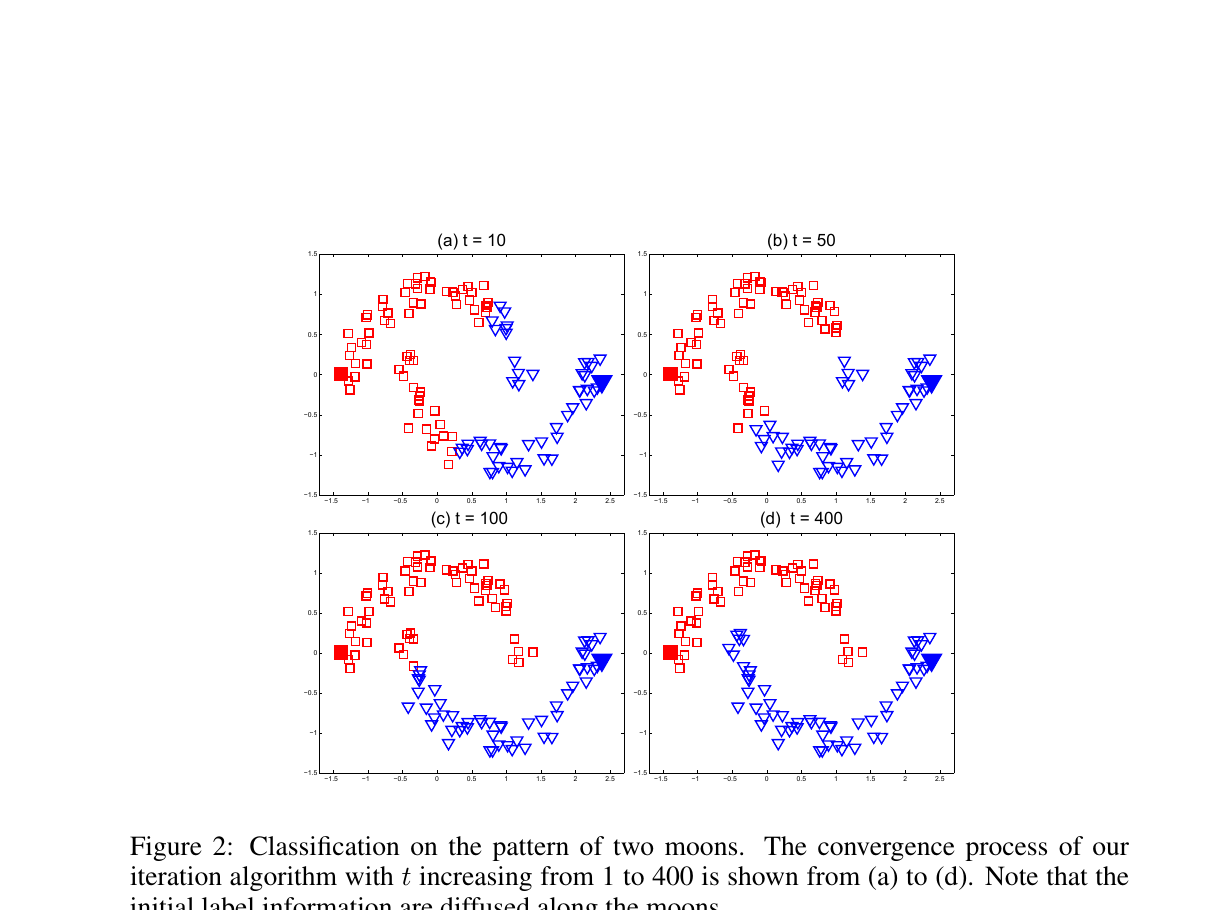
\includegraphics[width=\textwidth]{fig2_paper}\\[0.3em]
      {\footnotesize\paperfig{Figure 2: iterations 10, 50, 100 and 400}}
    \end{column}
    \begin{column}{0.41\textwidth}
      \begin{itemize}\small
        \item Each update carries class scores across one graph edge.
        \item After several updates, a label can influence distant points
              through a chain of strong similarities.
        \item The two moons emerge as coherent classes as scores spread
              along their curves.
      \end{itemize}
    \end{column}
  \end{columns}
  \note{About 60 seconds. Point to the two revealed labels in the figure.
  The rest of the points still matter because their positions shape the
  graph. Think of a chain A, B, C, D along one moon. If A is labeled, B gets
  a strong signal from A in one update. In later updates that signal travels
  through C to D. A and D can be far apart and still influence each other
  through those intermediate points. The picture shows this over four
  snapshots. The Gaussian gives nearby points stronger direct connections,
  and repeated updates make the longer structure visible in the scores.
  Dylan will now explain why those scores converge.}
\end{frame}

% ---------------------------------------------------------------- B: 2:00
\begin{frame}{The quiet hero is the normalization}
  \begin{columns}
    \begin{column}{0.52\textwidth}
      \begin{itemize}\small
        \item $S$ is similar to the row-stochastic $D^{-1}W$
              $\Rightarrow$ eigenvalues real, all in $[-1,1]$, top one $=1$
        \item $\alpha < 1$ makes $\alpha S$ a \textbf{contraction}:
              converges from \emph{any} start
        \item Neumann series: $\sum_i (\alpha S)^i = (I - \alpha S)^{-1}$
              $\Rightarrow F^{*} = (1-\alpha)(I-\alpha S)^{-1} Y$
        \item That inverse \emph{is} a diffusion kernel: a label reaches every
              point along every path, weighted $\alpha^{\text{path}}$ ---
              \textbf{global} consistency, literally
        \item Same shape as PageRank (damping, teleport); steps 1--2 are also
              spectral clustering's construction
      \end{itemize}
    \end{column}
    \begin{column}{0.44\textwidth}
      \vspace{0.2em}
      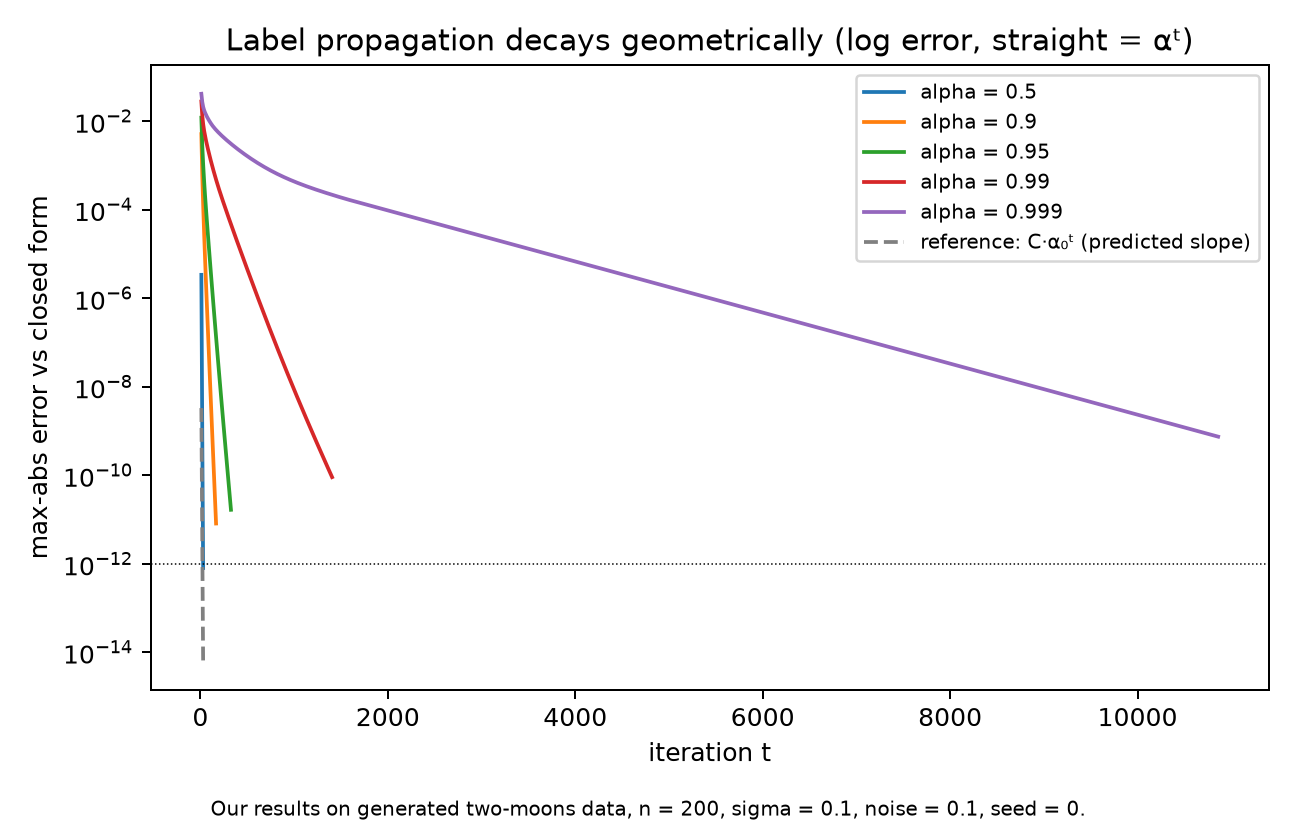
\includegraphics[width=\textwidth]{our_convergence_rate}\\[0.2em]
      {\footnotesize\ourfig{log error of the iteration per $\alpha$; straight $=$ geometric decay}}
    \end{column}
  \end{columns}
  \note{SAY (\textasciitilde65s): The algorithm looks like a heuristic. It isn't. Step two
  normalizes the similarity graph, and that quiet step is the whole ballgame. The normalized
  matrix is similar to a random walk matrix, so its eigenvalues live between minus one and
  one, and when alpha is below one, every pass shrinks the previous state. So the iteration
  converges no matter where you start, to a closed form, and because the sum of matrix powers
  telescopes to the inverse, that closed form is a diffusion kernel. One label reaches every
  point along every path in the graph, with alpha killing long paths. That's the global in
  global consistency. If this shape feels familiar, it's PageRank, same damping factor, same
  teleport idea. And the first two steps are exactly spectral clustering, so the graph
  machinery from our clustering lectures shows up inside a classifier.}
\end{frame}

\begin{frame}{Ridge regression wearing graph clothing}
  \begin{equation*}
    \mathcal{Q}(F) = \tfrac{1}{2}\sum_{ij} W_{ij}
    \Bigl\lVert \tfrac{F_i}{\sqrt{D_{ii}}} - \tfrac{F_j}{\sqrt{D_{jj}}} \Bigr\rVert^{2}
    \;+\; \mu \sum_i \lVert F_i - Y_i \rVert^{2}
  \end{equation*}
  \vspace{-0.5em}
  \begin{columns}
    \begin{column}{0.52\textwidth}
      \begin{itemize}\small
        \item smoothness energy + fidelity to the known labels,
              $\mu$ is the dial \; ($\alpha = \tfrac{1}{1+\mu}$)
        \item $\partial\mathcal{Q}/\partial F = 0$ \emph{is} the fixed point:
              iterate $=$ solve $(I-\alpha S)F = \beta Y$ $=$ minimize $\mathcal{Q}$
        \item convex quadratic $\Rightarrow$ unique answer
        \item our verification: gradient zero to $2\!\times\!10^{-17}$,
              18/18 perturbations raise $\mathcal{Q}$,
              stopping error $=$ tol$/ (1{-}\alpha)$ exactly
      \end{itemize}
    \end{column}
    \begin{column}{0.44\textwidth}
      \vspace{0.3em}
      {\footnotesize
      \begin{tabular}{@{}lll@{}}
        \toprule
        $\alpha$ & iters & diff vs solve\\
        \midrule
        0.5   & 29    & $8.1\mathrm{e}{-}13$\\
        0.9   & 167   & $8.2\mathrm{e}{-}12$\\
        0.99  & 1405  & $9.1\mathrm{e}{-}11$\\
        0.999 & 10860 & $7.5\mathrm{e}{-}10$\\
        \bottomrule
      \end{tabular}}\\[0.4em]
      {\footnotesize\ourfig{$\alpha$-sweep on generated two-moons data}}
    \end{column}
  \end{columns}
  \note{SAY (\textasciitilde60s): Why should that fixed point be the right answer? Because
  it's the exact minimizer of an honest objective. Half the graph smoothness energy, plus mu
  times the squared distance to the labels we actually know. First term says predictions
  should change slowly along edges, second says don't drift from the clamped labels. That's
  the ridge regression story from every regularization lecture, with the graph Laplacian in
  place of the weight penalty, and mu trading them off. Take the derivative, set it to zero,
  substitute one over one plus mu, and the paper's iteration falls out. So iterating, solving
  a linear system, and minimizing an objective are the same thing. And we didn't take that on
  faith: on our data the gradient at the claimed minimum is zero to machine precision, every
  random nudge we tried made the objective worse, and the error curve falls exactly as fast
  as the theory says.}
\end{frame}

% ---------------------------------------------------------------- C: 2:00
\begin{frame}{What the paper's experiments show}
  \begin{columns}
    \begin{column}{0.62\textwidth}
      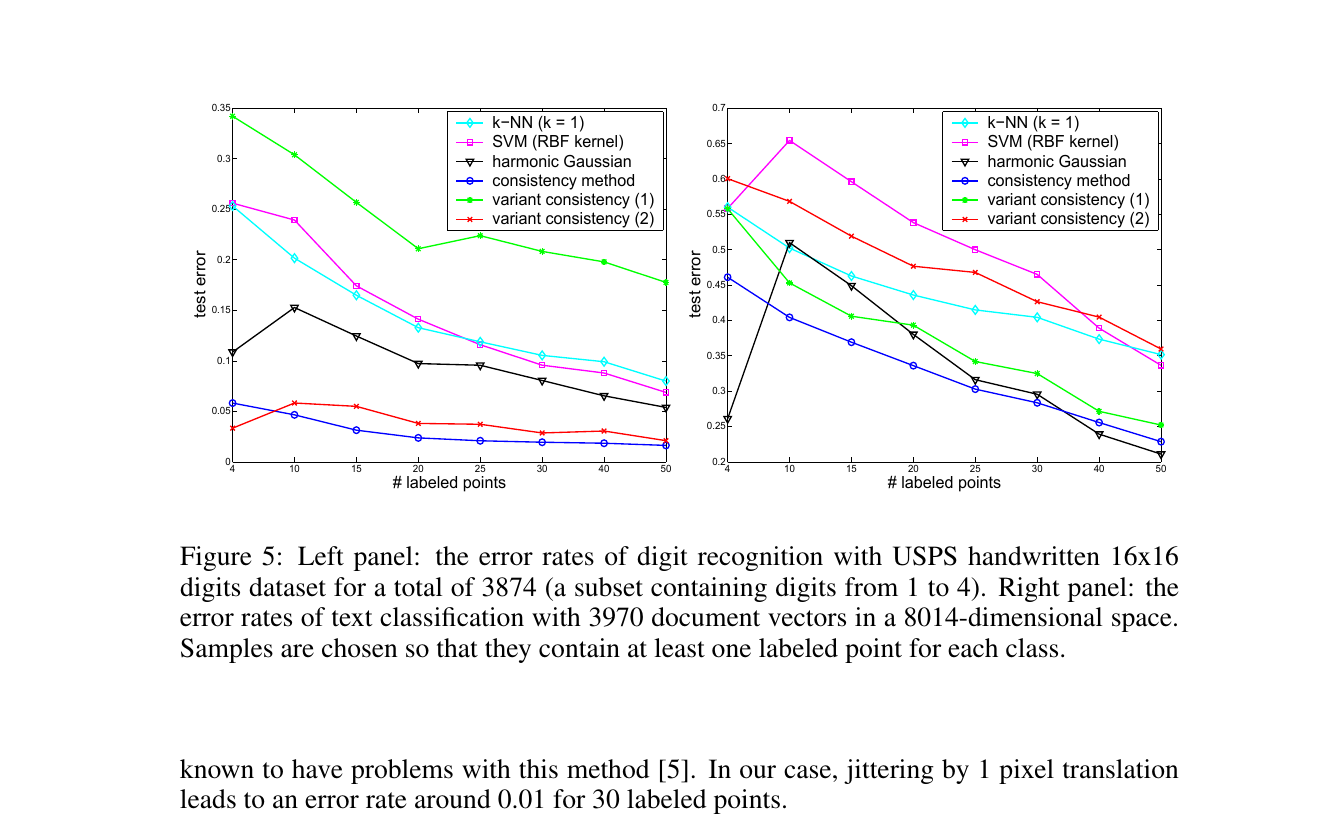
\includegraphics[width=\textwidth]{fig5_paper}\\[0.2em]
      {\footnotesize\paperfig{Figure 5: digits (left), text (right), mean of 100 trials}}
    \end{column}
    \begin{column}{0.34\textwidth}
      \vspace{0.8em}
      \begin{itemize}\scriptsize
        \item $\geq$1 label per class, error on unrevealed points
        \item digits: LGC clearly beats 1-NN and RBF SVM
        \item text: the harmonic method wins at some label budgets ---
              no universal dominance
        \item each method tuned to its own optimum: tuning with few labels
              stays unresolved
      \end{itemize}
    \end{column}
  \end{columns}
  \note{SAY (\textasciitilde60s): The authors illustrate the method on two moons, then test it
  on handwritten digits and newsgroup text. Figure 5 shows the number of revealed labels along
  the bottom and the error on unrevealed points on the vertical axis. Lower is better. Each
  point averages a hundred trials, with at least one label per class. On digits, the
  consistency method has substantially lower error than nearest neighbor and SVM. On text, the
  related harmonic method does better at some label budgets. The paper also compares methods at
  their respective optimal parameters, so choosing those parameters with very few labels
  remains an open practical question.}
\end{frame}

\begin{frame}{Our paired two-moons experiment}
  \begin{columns}
    \begin{column}{0.60\textwidth}
      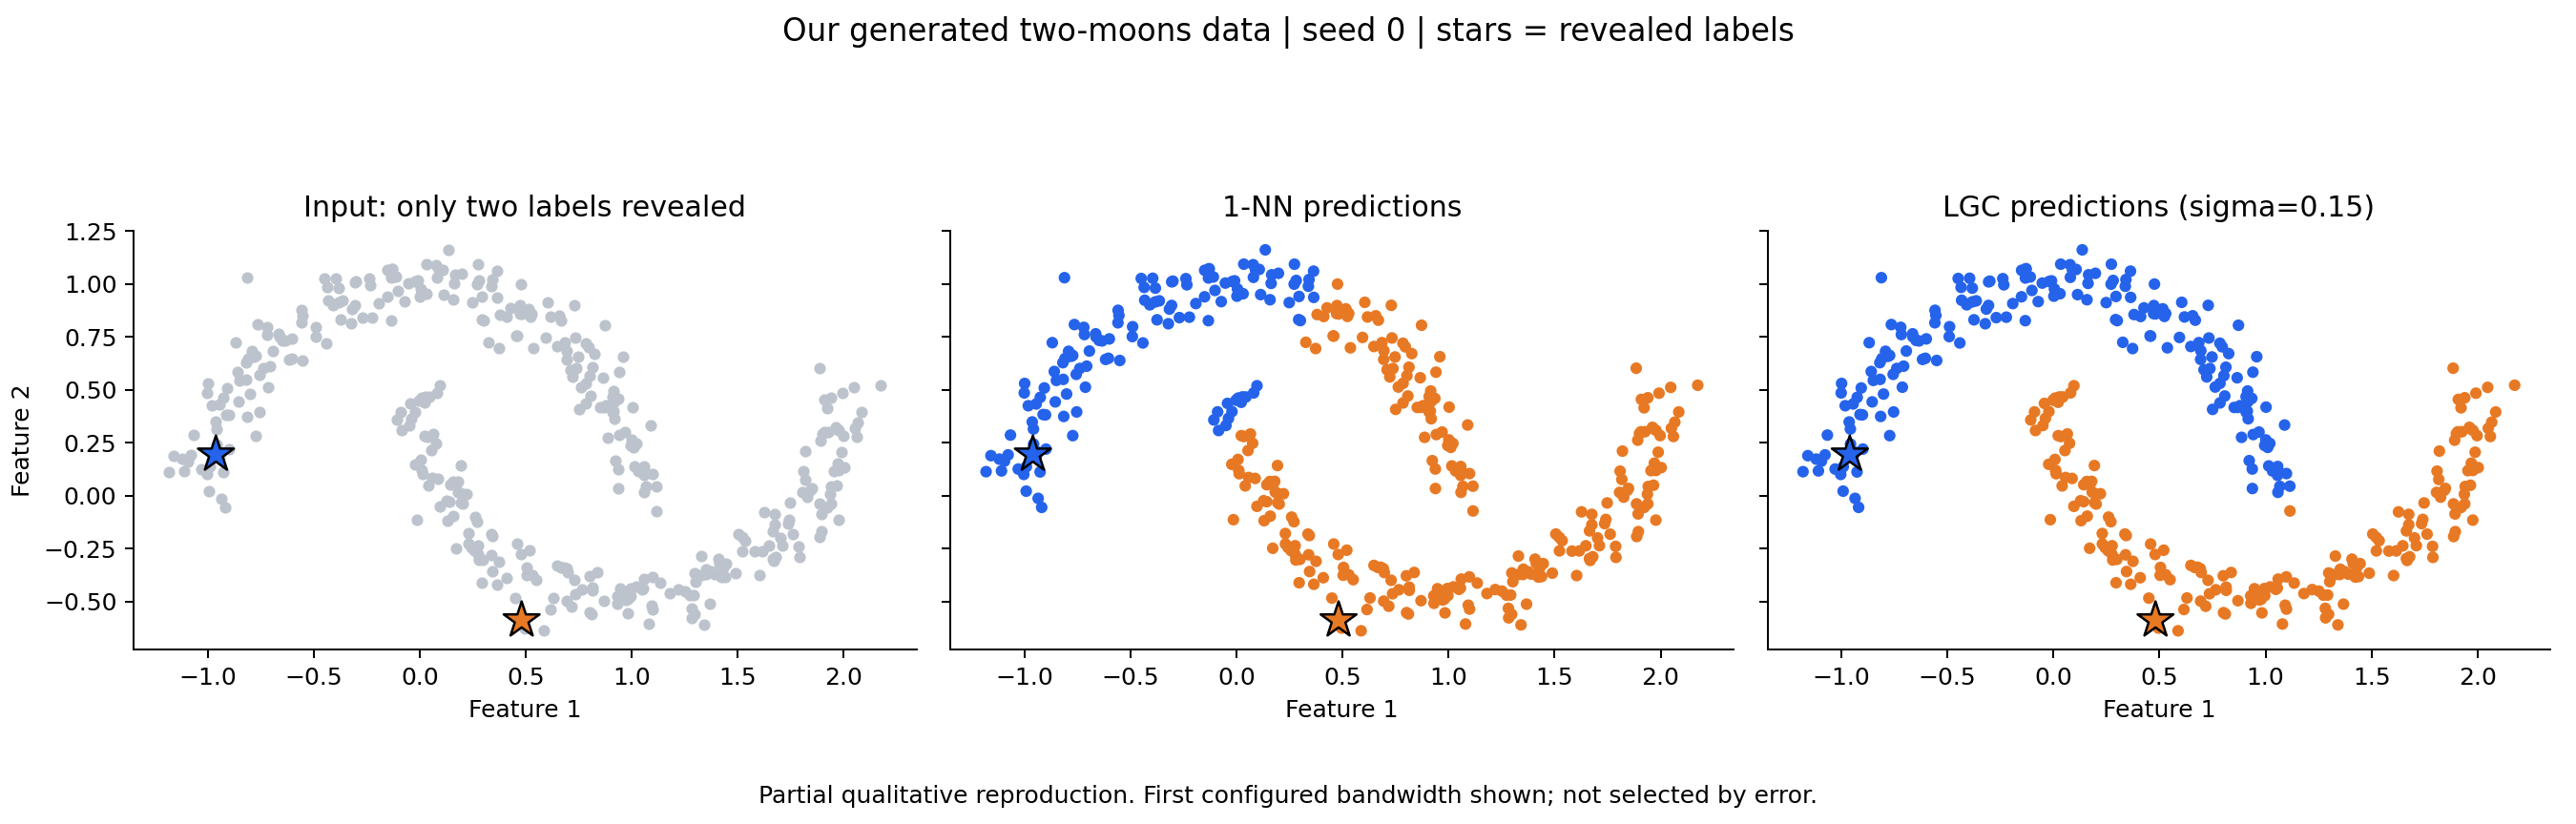
\includegraphics[width=\textwidth]{our_moons_example}\\[0.2em]
      {\footnotesize\ourfig{seed 0: 1-NN cuts across the moons; LGC follows the arcs}}
    \end{column}
    \begin{column}{0.36\textwidth}
      \vspace{0.4em}
      \begin{itemize}\small
        \item 10 seeds, 400 points, \textbf{one} revealed label per class
        \item mean error: 1-NN \textbf{22.36\%} $\to$ LGC \textbf{0.45\%}
              ($\sigma{=}0.15$, $\alpha{=}0.99$)
        \item LGC better in every paired trial at 0.15
        \item $\sigma{=}0.6$: error \textbf{32.59\%} --- bandwidth can
              bridge the moons
      \end{itemize}
    \end{column}
  \end{columns}
  \note{SAY (\textasciitilde60s): We generated ten two-moons datasets of four hundred points
  each and revealed one label per moon. Both methods used the same two labels in each trial.
  On this example, nearest neighbor cuts across the moons, while LGC can spread the label
  signal along the arcs using the unrevealed points. Across all ten trials, nearest neighbor
  averaged 22.36 percent error. At our fixed bandwidth, LGC averaged 0.45 percent. At a much
  wider bandwidth, its error climbed to 32.59 percent. Wider affinities can connect points
  across the moons and blur the class boundary. That sensitivity matters when only a few
  labels are available to guide the choice.}
\end{frame}

% ---------------------------------------------------------------- D: 1:15
\begin{frame}{Where this breaks --- and what's next}
  \todo{own this frame: critique + extensions. Raw material approved in
  docs/c\_paper\_evidence.md (limitations 1--8) and results/convergence\_check\_summary.md
  (decay-slope nuance, row-scaling equivalence).}
  \vspace{0.5em}
  \begin{itemize}
    \item \todo{D: suggest --- model selection with almost no labels is still open;
          our own $\sigma$ sweep is evidence, not decoration}
    \item \todo{D: transductive assumption: graph built on the test points themselves}
    \item \todo{D: dense $n \times n$ solve --- cost at scale, what changes for 100k points}
  \end{itemize}
\end{frame}

\begin{frame}{Conclusion}
  \todo{D: one slide, four sentences max. Suggested spine: one idea (smooth on the graph
  $=$ semi-supervised learning), one proof we did ourselves (iterate $=$ solve $=$
  minimize, verified to machine precision), one honest limit (bandwidth and budgets),
  one line on why it still matters (it's PageRank for labels).}
\end{frame}

% ---------------------------------------------------------------- appendix
\appendix
\begin{frame}{Backup: the equation check (B)}
  \begin{itemize}\small
    \item \S2's closing claim: transpose variant ``equivalent to $(D-\alpha W)^{-1}DY$''
          --- as matrices it is \textbf{not} (measured relative gap $0.82$)
    \item the identity that holds (to $2.5\!\times\!10^{-15}$):
          $(I-\alpha P^{\top})^{-1}Y = D\,(D-\alpha W)^{-1}Y$
    \item pre-multiplying by $D$ is a positive \emph{row rescaling} $\Rightarrow$
          argmax unchanged --- ``equivalent for classification'' survives,
          the displayed equation doesn't
    \item all operator variants shift $\leq 6/200$ toy predictions:
          classification is robust to normalization choice
    \item integration receipt: A's core vs B's closed form, 0/400 label differences,
          all ten seeds (\texttt{results/protocol\_check.csv})
  \end{itemize}
\end{frame}

\begin{frame}{Backup: bandwidth sweep (ours)}
  \begin{center}
    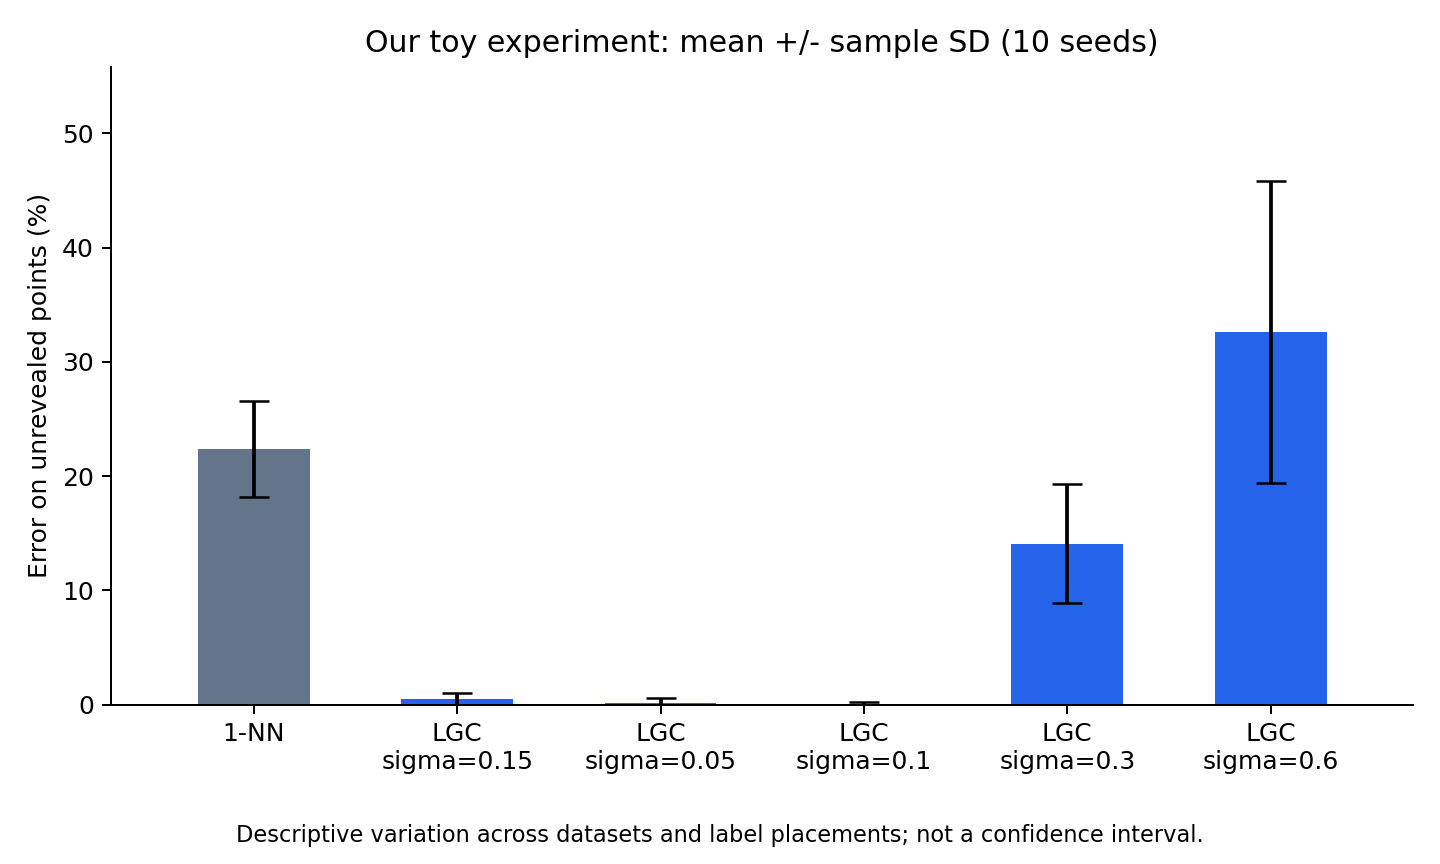
\includegraphics[width=0.62\textwidth]{our_error_summary}\\[0.2em]
    {\footnotesize\ourfig{mean error $\pm$ sample SD over 10 seeds}}
  \end{center}
\end{frame}

\begin{frame}{Sources}
  \begin{itemize}\small
    \item Zhou, Bousquet, Lal, Weston, Sch\"olkopf. \emph{Learning with Local and Global
          Consistency.} NIPS 2003, 321--328. (Figures 2 and 5: the paper, cited for
          coursework use)
    \item Our code, data and figures: \texttt{github.com/IliyasBaish/comp3314-group28}
          (\texttt{experiments/}, \texttt{results/}, \texttt{src/})
    \item Ng, Jordan, Weiss (NIPS 2001); Zhu, Ghahramani, Lafferty (ICML 2003) ---
          cited via the paper's Sections 2--4
  \end{itemize}
\end{frame}

\end{document}
